%===================================== CHAP 7 =================================

\chapter{Project life cycle}
\label{ch:project_lifecycle}

\section{Planning and research}
\label{sec:project_lifecycle-planning_and_research}

This section provides a general description of the planning and research phase of the process. It attempts to capture the main aspects of the process and work done.

\subsection{Planning phase}
\label{subsec:project_lifecycle-planning_and_research-planning_phase}

The planning phase of this project consisted mainly of defining the outer scope of the project. That included negotiating core requirements with the customer, as well as research on relevant technologies and existing solutions. A report document structure was also created, and both the introduction and parts of the prestudies chapter were written. The group also had to define internal meeting \& communication terms.

\subsubsection{Goals}
\label{subsec:project_lifecycle-planning_and_research-planning_phase-goals}

\begin{enumerate}
\item Discuss and define the project description.
\item Define core functional requirements.
\item Research previous and similar work.
\item Select development strategy and team organization.
\item Define development and communication environment.
\end{enumerate}

\subsubsection{Discussion}
\label{subsec:project_lifecycle-planning_and_research-planning_phase-discussion}

All of the goals were achieved in this iteration. The work required during this phase was somewhat overestimated. This was mainly due to reaching agreement with the customer quickly, and the group working well together from the beginning. In total, 180 hours were spent on the planning phase, out of the 240 hours initially planned. The remaining 60 hours probably could have been used more efficiently. A portion of this time was used to construct the outlines of the report, but the remainder should have been allocated to the research phase. 

\subsection{Research phase}
\label{subsec:project_lifecycle-planning_and_research-research_phase}

The research phase of this project was initially introduced due to the option of using Apollo (section \ref{subsec:prestudies-existing_solutions-apache_apollo}) as the core of the system. Thus, the only goal of this phase was to do extensive research, and find out whether to expand Apollo or develop a new system. The research work was split into different focal points, in order to assess all the major points of uncertainty (table \ref{tab:risk_analysis_apollo}). At the end of this phase, a decision had to be made. This was anchored in our risk analysis, where choosing a too complex architectural design would trigger the group to fall back to an alternative solution.

\subsubsection{Discussion}
\label{subsec:project_lifecycle-planning_and_research-research_phase-discussion}

The group were able to reach a decision regarding the system. The choice was a result of the repeated evaluation of the focal points in the associated risk analysis (table \ref{tab:risk_analysis_apollo}). Two of the members were able to get a fairly good overview of the Scala programming language. However, problems arose when the code base was thoroughly inspected. It proved to be massive, and required a lot more research to get a good enough understanding. That also affected the time it would take to implement additional protocol modules. After hours of discussion, Apollo was ultimately discarded. The following arguments made the basis for the final decision:

\begin{itemize}
\item The group did not have sufficient understanding of the asynchronous workings of the embedded Scala classes
\item Apollo is a fairly large and complex project, that requires a lot of effort to get a complete grasp on.
\item Even though Apollo has a very dynamic architecture  allowing extension by adding custom Java archived components, it requires thorough understanding of the core application.
\item The group could not justify proceeding with Apollo, given the time available and the risk of not being able to gain a proper understanding in time to complete a working product.
\end{itemize}

A large amount of time had been invested in this research phase, and one might argue that it impacted the product development in a negative way. This is mainly due to lost development time. The positive aspect of it were that several good practices and ways to implement a brokering system were learned.. Additionally, the group might not have been able to finish a working product in time, had the decision been to proceed with Apollo before understanding the amount of effort required.

\section{Development}
\label{subsec:project_lifecycle-development}

This section describes the iterations devoted to development and testing of the software. The following sections includes a general explanation of each sprint, as well as issues the group faced. With the development phase of the project, burndown charts were introduced. This was made in combination with a list of the tasks to be executed for each sprint, as well as the time usage on each task. Tasks that were not completed in a sprint were transferred to the next sprint. The tasks functioned as an interpretation of sprint backlogs. They do not directly consider the requirements or user stories, but rather work packages from the development part of the WBS(\ref{subsec:process_and_methodology-resource_management-work_breakdown}),  The charts does not consider time used on the report, peer evaluation and meetings with the customer.

\subsection{Sprint 1}
\label{subsec:project_lifecycle-development-sprint_1}

This was the first of the development cycles. It consisted mainly of setting up the development environment, and constructing the base project templates and structure. At the end of the sprint, the goal was to have a solid foundation both for the broker and web interface.

\subsubsection{Goals}
\label{subsec:project_lifecycle-development-sprint_1-goals}

\begin{center}
\begin{table}[ht!]
\small
\centering
\begin{tabular}{|p{10cm}|p{2cm}|}
\hline
\rowcolor{lightgray}
 \textbf{Task} & \textbf{Status} \\
\hline
\rowcolor{green!30}
 Initial JavaScript modules for admin console & Completed  \\
 \rowcolor{green!30}
 Template for admin console & Completed \\ 
 \rowcolor{green!30}
 Web server instance & Completed \\ 
 \rowcolor{green!30}
 Decide on technology stack & Completed \\ 
 \rowcolor{green!30}
 Project structure & Completed \\
 \rowcolor{green!30}
 Create initial core service architecture & Completed \\
 \rowcolor{green!30}
 Initial database design and relational schema & Completed \\
\hline
\end{tabular}
\caption{Goal achievement for sprint 1}
\label{tab:sprint 1, goals}
\end{table}
\end{center}

\begin{center}
  \begin{figure}[htbp!]
    \makebox[\textwidth]{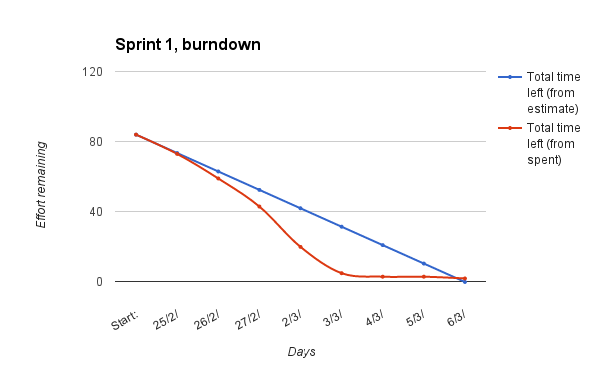
\includegraphics[width=\textwidth]{fig/burndown/sprint1Burndown.png}}
    \caption{Burndown chart for sprint 1}
    \label{fig:sprint 1, burndown}
  \end{figure}
\end{center}

\subsubsection{Discussion}
\label{subsec:project_lifecycle-development-sprint_1-discussion}

As expected, the first development sprint was fairly straight forward. The structure of the project was strongly influenced by Apollo. That made the work of defining the structure and base templates simpler, and less time consuming than first expected. Only one of the tasks were still in progress at the end of the sprint. However, given the progress on the task, the group assumed that only a couple of hours remained on it. There were also some minor deviations in the time spent on tasks versus the time that was estimated.

\subsection{Sprint 2}
\label{subsec:project_lifecycle-development-sprint_2}

The major goals of sprint 2 was to get initialize the first draft of the web interface, as well as identify and implement support for processing incoming WSN messages. The midterm report was also due at the end of this sprint.

\subsubsection{Goals}
\label{subsec:project_lifecycle-development-sprint_2-goals}

\begin{table}[ht!]
\small
\centering
\begin{tabular}{ | p{10cm} | p{2cm} |}
\hline
\rowcolor{lightgray}
 \textbf{Task} & \textbf{Status} \\
\hline
\rowcolor{orange!40}
Structurize RESTapi & Not completed \\
\rowcolor{green!30}
Mockup for topics pane & Completed \\
\rowcolor{green!30}
JavaScript for creating tables for each topic the broker has a subscription on & Completed \\
\rowcolor{green!30}
Models for topics/stats & Completed \\
\rowcolor{orange!40}
Stats functionality	& Not completed \\
\rowcolor{green!30}
Identify WS-Nu components needed to intercept an incoming message & Completed \\
\rowcolor{orange!40}
Identify WS-Nu components needed to create and deliver a valid WSN soap message & Not completed \\
\rowcolor{orange!40}
Set up the needed components to receive and handle incoming message, and pass it to the CoreService	& Not completed \\
\rowcolor{green!30}
Create initial core service architecture & Completed \\
\hline
\end{tabular}
\caption{Goal achievement for sprint 2}
\label{tab:sprint 2, goals}
\end{table}


\begin{center}
  \begin{figure}[ht!]
    \makebox[\textwidth]{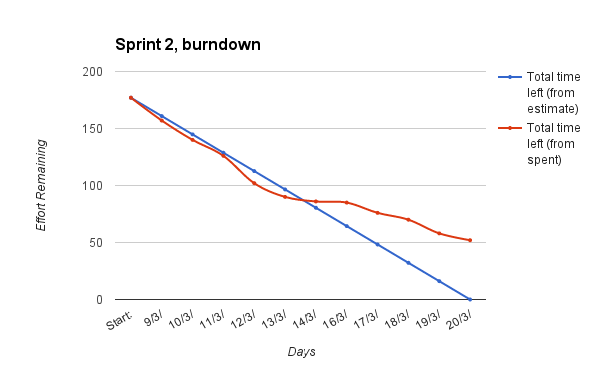
\includegraphics[width=0.9\textwidth]{fig/burndown/sprint2Burndown.png}}
    \caption{Burndown chart for sprint 2}
    \label{fig:sprint 2, burndown}
  \end{figure}
\end{center}

\subsubsection{Discussion}
\label{subsec:project_lifecycle-development-sprint_2-discussion}

At the start of this sprint, quite a bit of content lacked on the report in order to deliver a satisfying mid term version. That prompted the group to dedicate a lot of time to the report. Some of the work regarding WSN had to pushed to the next sprint, along with other, less important tasks. Obviously, it would have been preferable to finish the work on time. However, quite a lot of time was left before a functional version of the WSN broker were to be completed. Thus, transferring the packages to the next sprint, seemed okay time-wise. Also, the customer seemed happy with the progress, and was satisfied with the topic handling part of the user interface.

\subsection{Sprint 3}
\label{subsec:project_lifecycle-development-sprint_3}

Only 60 hours were initially scheduled for sprint 3. This was due to Easter, and that three of the group members were on a class trip. The main goals of the sprint were topic and subscription mapping. That included both the logic of it, and passing it to the web interface. The incomplete packages from sprint 2 were also included.

\subsubsection{Goals}
\label{subsec:project_lifecycle-development-sprint_3-goals}

\begin{table}[ht!]
\small
\centering
\begin{tabular}{ | p{10cm} | p{2cm} |}
\hline
\rowcolor{lightgray}
 \textbf{Task} & \textbf{Status} \\
\hline
\rowcolor{orange!40}
Create mockup for config pane, including topic mapping & Not completed \\
\rowcolor{green!30}
Structurize RESTapi & Completed \\
\rowcolor{orange!40}
Stats functionality & Not completed \\
\rowcolor{green!30}
Identify WS-Nu components needed to create and deliver a valid WSN soap message & Completed \\
\rowcolor{orange!40}
Set up the needed components to receive and handle incoming message, and pass it to the CoreService & Not completed \\
\rowcolor{orange!40}
Subscription & Not completed \\
\hline
\end{tabular}
\caption{Goal achievement for sprint 3}
\label{tab:sprint 3, goals}
\end{table}

\begin{center}
  \begin{figure}[ht!]
    \makebox[\textwidth]{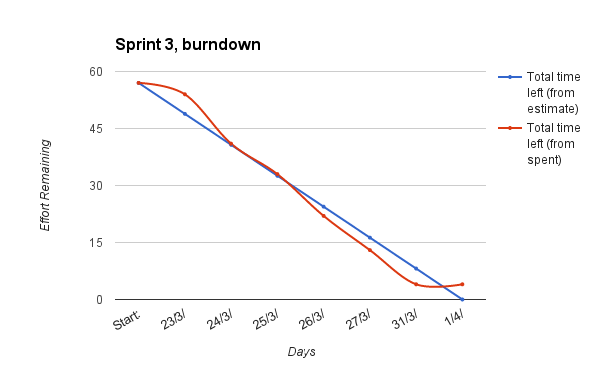
\includegraphics[width=\textwidth]{fig/burndown/sprint3Burndown.png}}
    \caption{Burndown chart for sprint 3}
    \label{fig:sprint 3, burndown}
  \end{figure}
\end{center}

\subsubsection{Discussion}
\label{subsec:project_lifecycle-development-sprint_3-discussion}

At this point, the progress and status of the project was not ideal. After the sprint, some of the smaller packages were still unfinished. They were left untouched due to the importance of the other parts of the system. As the system was shaping up as quite complex, more time was used to identify where and how to implement the different parts. This was obviously an issue, as it decreased the amount of code being added. However, the subscription and topic handling were almost completed at the end of the sprint. Thus, no remedial actions were taken at the time, but the issues were kept in mind.


\subsection{Sprint 4}
\label{subsec:project_lifecycle-development-sprint_4}

The focus of this sprint was initially to finalize the implementation of WSN. Additionally, a lot of work had to be put into the report, the peer evaluation and general research on WSN. The group realized that completing the WSN implementation was not doable at the end of the sprint. The main focus was thus to finalize the subscription and publish parts. Lastly, a major issue with sprint 4 was major deliveries in other courses, that took much more time than anticipated.

\subsubsection{Goals}
\label{subsec:project_lifecycle-development-sprint_4-goals}

\begin{table}[ht!]
\small
\centering
\begin{tabular}{ | p{10cm} | p{2cm} |}
\hline
 \rowcolor{lightgray}
 \textbf{Task} & \textbf{Status} \\
\hline
\rowcolor{green!30}
Create mockup for config pane, including topic mapping & Completed \\
\rowcolor{green!30}
Stats functionality	& Completed \\
\rowcolor{green!30}
Set up the needed components to receive and handle incoming message, and pass it to the CoreService	& Completed \\
\rowcolor{orange!40}
Finish up custom web services and commandproxies that allow interception of requests in WS-Nu	& Not completed \\
\rowcolor{green!30}
Create a first draft of OKSE SubscriptionManager & Completed \\
\rowcolor{green!30}
Create a first draft of OKSE Subscriber and Publisher objects & Completed \\
\rowcolor{orange!40}
Create support methods for transformation to and from WS-Nu request and message representation	& Not completed \\
\rowcolor{green!30}
Create a first draft for OKSE Topic management & Completed \\
\rowcolor{orange!40}
Start looking into MQTT	& Not completed \\
\hline
\end{tabular}
\caption{Goal achievement for sprint 4}
\label{tab:sprint 4, goals}
\end{table}

\begin{center}
  \begin{figure}[ht!]
    \makebox[\textwidth]{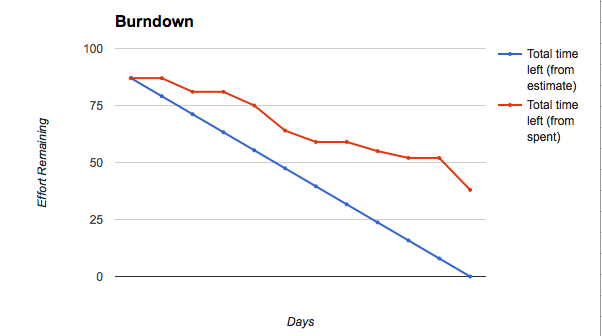
\includegraphics[width=\textwidth]{fig/burndown/sprint4Burndown.png}}
    \caption{Burndown chart for sprint 4}
    \label{fig:sprint 4, burndown}
  \end{figure}
\end{center}

\subsubsection{Discussion}
\label{subsec:project_lifecycle-development-sprint_4-discussion}

The two main reasons for this sprint not containing the planned workload were major deliveries in other courses, as well as group members being in Oslo for summer job interviews.
Due to the challenges discussed in the previous sprint, the group had to discuss the priority of requirements with the customer. The solution was to re-prioritize the requirements of MQTT and AMQP support. The result became that AMQP now was the first-in-line protocol to be implemented, bumping MQTT down at a lower priority level. Previously, both AMQP and MQTT had been at the same priority level. That led to a rework of the schedule for the remaining sprints. A lot of time was used for research on the remaining parts of WSN this sprint, along with a lot of report work. WSN proved to be more and more comprehensive and complex, and more code was needed for the implementation than first expected. Even with this in mind, the group still somewhat underperformed. Too little time was dedicated to actual development work. Thus, the group realized that a lot more time had to be scheduled for the following sprints. A new work plan was made for the remaining sprints.


\begin{center}
\begin{table}[ht!]
\centering
\small
\begin{tabular}{ | m{0.4cm} | m{3.3cm}| m{0.7cm} | m{0.9cm} | m{0.9cm}| m{4.4cm} |} 
\hline
\rowcolor{lightgray}
\textbf{ID} & \textbf{Task name} & \textbf{Days} & \textbf{Start} & \textbf{End} & \textbf{Notes} \\
\hline
\textbf{6} & \textbf{Iteration 4} & \textbf{9} & \textbf{07.04} & \textbf{17.04} & \textbf{Monday of Orthodox Easter} \\
 & Stats functionality & & & & \\
 & Subscribe and publish  & & & & \\
\hline
\textbf{7} & \textbf{Iteration 5} & \textbf{9} & \textbf{20.04} & \textbf{30.04} & \textbf{First of May} \\
 & AMQP implementation & & & & \\
 & Finalize WSN & & & & \\
\hline 
\textbf{8} & \textbf{Iteration 6} & \textbf{9} & \textbf{04.05} & \textbf{15.05} & \textbf{Ascension day} \\
 & Finalize AMQP & & & & \\
\hline
\textbf{9} & \textbf{End phase} & \textbf{8} & \textbf{22.05} & \textbf{30.05} & \\
 & Documentation & & & & \\
 & Component test & & & & \\
 & Acceptance test & & & & \\
 & System test & & & & \\
 & Delivery & & 30.05 & 30.05 & Delivery day \\
\hline
\end{tabular}
\caption{Updated work plan}
\label{tab:workplan, revised}
\end{table}
\end{center}

\subsection{Sprint 5}
\label{subsec:project_lifecycle-development-sprint_5}
At the start of sprint 5, lectures and tasks were completed in other courses. That meant that all resources could be devoted to the project. Considering the issues explained in the previous sprint, as well as the fact that the time left was getting short, a lot of work was scheduled for this sprint. The main task for this sprint was finalizing the most important aspects of WSN, as well as getting an overview of AMQP.

\subsubsection{Goals}
\label{subsec:project_lifecycle-development-sprint_5-goals}

\begin{table}[ht!]
\small
\centering
\begin{tabular}{ | p{10cm} | p{2cm} |}
\hline
 \rowcolor{lightgray}
 \textbf{Task} & \textbf{Status} \\
\hline
\rowcolor{green!30}
Create support methods for transformation to and from WS-Nu request and message representation & Completed \\
\rowcolor{green!30}
Get an overview of AMQP standard & Completed \\
\rowcolor{green!30}
Create WSNRegistrationManager class and implement needed methods & Completed \\
\rowcolor{orange!40}
Research, implement and test support and features needed for WSN to use different dialects	& Not completed \\
\rowcolor{orange!40}
Start on writing the developer manual & Not completed \\
\rowcolor{orange!40}
Improve source code documentation & Not completed \\
\rowcolor{orange!40}
Perform component testing of WSNotification	& Not completed \\
\rowcolor{orange!40}
Create subscribers-pane	& Not completed \\
\rowcolor{green!30}
General fix in UI & Completed \\
\rowcolor{green!30}
Update GUI to new methods in CoreService & Completed \\
\rowcolor{green!30}
AMQP sendMessage & Completed \\
\rowcolor{green!30}
Refactorization of JS & Completed \\
\rowcolor{orange!40}
AMQP subscribe & Not completed \\
\rowcolor{green!30}
AMQO Driver.stop() & Completed \\
\hline
\end{tabular}
\caption{Goal achievement for sprint 5}
\label{tab:sprint 5, goals}
\end{table}

\begin{center}
  \begin{figure}[ht!]
    \makebox[\textwidth]{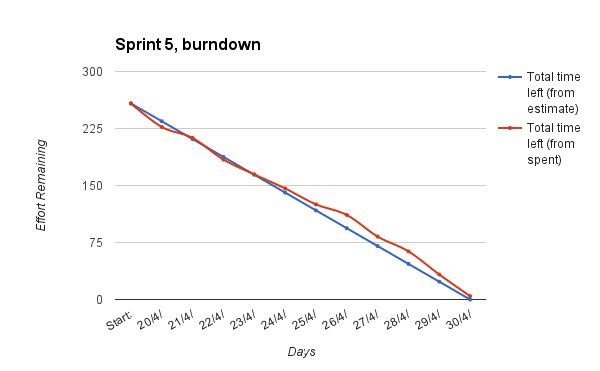
\includegraphics[width=\textwidth]{fig/burndown/sprint5Burndown.png}}
    \caption{Burndown chart for sprint }
    \label{fig:sprint 5, burndown}
  \end{figure}
\end{center}


\subsubsection{Discussion}
\label{subsec:project_lifecycle-development-sprint_5-discussion}

Almost all resources were assigned to implementation this sprint, and a lot of work was done on the system. Although a fair amount of the packages weren't fully completed at the end, WSN only lacked proper testing before completion. A lot of work had also been done on AMQP, and the protocol proved much simpler than WSN. Thus, the project was back on schedule, and it seemed likely that the implementation would be completed after the next sprint.

\subsection{Sprint 6}
\label{subsec:project_lifecycle-development-sprint_6}

\subsubsection{Goals}
\label{subsec:project_lifecycle-development-sprint_6-goals}

\subsubsection{Discussion}
\label{subsec:project_lifecycle-development-sprint_6-discussion}

\subsection{Discussion}

[REMEMBER TO ADD THE RELEASE BURNDOWN]

\section{Final phase}

\clearpage